% !TEX encoding = UTF-8 Unicode

\documentclass[BIF,Seminar,english]{twbook}
\usepackage[utf8]{inputenc}
\usepackage[T1]{fontenc}

\usepackage{minted}
\makeatletter
\providecommand\listacroname{}
\@ifclasswith{twbook}{english}
{%
    \renewcommand\listoflistingscaption{List of source codes}
    \renewcommand\listacroname{List of Abbreviations}
}{%
    \renewcommand\listoflistingscaption{Quellcodeverzeichnis}
    \renewcommand\listacroname{Abk�rzungsverzeichnis}
}
\makeatother

\usepackage{blindtext}


\title{Interface segregation principle}
\author{Peter Oettl}
\studentnumber{1910257146}
\supervisor{DI Wolfgang Berger}
\place{Wien}

\begin{document}

\maketitle
\chapter{SOLID principles}

These principles describe practices for software development with considerations for maintaining and extending as the project grows. Adopting these practices can also contribute to avoiding code smells, refactoring code, and Agile or Adaptive software development. \cite{SOLID}



\section{S - Single Responsiblity Principle}

The single responsibility principle describes that one class is only supposed to handle one topic. This principle ensures that a class exists only for a single reason but can have multiple methods to carry out distinct functions.\cite{IntroductionSOLID}

\section{O - Open Close Principle}


This principle ensures that objects should be open for extension but closed for any modification. This principle ensures that the code is easily extensible without editing or rewriting the existing codebase. Designing software applications using this principle ensures extensibility and the reusability of objects.\cite{IntroductionSOLID}

\section{L - Liskov Substitution Principle}

This principle describes that if a section of your code is extending a superclass, then all subclasses of the superclass should be able to replace the superclass in your code. A part of your code does not have to know which class it is, since it is a superclass subclass. The use-case of this principle ensures the easy integration of classes.\cite{IntroductionSOLID}


\section{I - Interface Segregation Principle}

The interface segregation principle simply means that larger interfaces should be split into smaller ones. This ensures that implementing classes only need to be concerned about the methods that are of interest and necessary. \cite{ISP}

\section{D - Dependency Inversion Principle}

The dependency inversion principle guarantees that classes should not depend on solid classes but should only depend on an abstraction of classes. By following this approach, makes the replacing and changing of modules and classes or services more simple. The dependency inversion principle makes changing dependencies easier.\cite{IntroductionSOLID}


\chapter{Interface segregation principle}

\begin{figure}[!htbp]
\centering
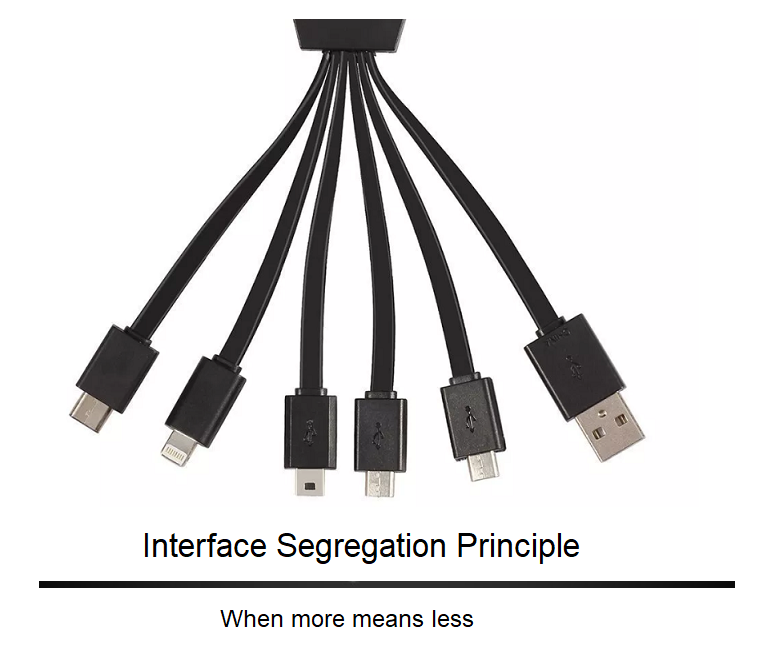
\includegraphics[width=0.5\linewidth]{PICs/ISP}
\caption{Interface segregation principle}\label{Abb1}
\end{figure}


\section{Interface}

An interface is a blueprint for an object and what it is capable of. In Object-Oriented Programming, an Interface is a description of all functions that an object must have to be a specified Interface. Again, as an example, anything that "ACTS LIKE" a light, should have a turnOn() method and a turnOff() method. The purpose of interfaces help developers to enforce these properties and to know that an object of TYPE T must have functions and properties called X, Y, Z, etc. \cite{utah}


\section{ISP}

\begin{center} 
 ``Clients should not be forced to depend upon interfaces that they do not use.''\cite{ISP}\newline
\end{center} 

This principle was developed by Robert C. Martin while working at Xerox as a consultant. Martin was in charge of developing a new printing management system that could carry out tasks concurrently, which was new by the time.\cite{solidISP}

During the development process, Martin noticed that smaller changes in the design caused larger deployments. In some same cases caused deployments on modules out of the scope of the change. The problem was mainly caused by a large fat interface used throughout all the modules of the system.\cite{solidISP}

This principle is simple and clear, interfaces should not be forced to implement methods that they do not use. It has the main goal of limiting the scope of future changes. However, it is very difficult, in the first iterations, to identify the critical parts of your solution that will violate the principle.\cite{solidISP}


\section{Problem with will be solved with the ISP}
With ISP you can prevent overloaded interfaces that force the client to implement a method that is not required. The client ends up implementing a usefulness method, in other words, a method that has no meaning to the client. These circumstances decrease the readability of the code and also confuses every other developer who will work with the code.
The client interface ends up violating SRP sometimes since it might perform some action that is not related to it.\cite{csharpsolid}


\newpage

\chapter{Practical Example}

In the first example, the Ostrich class is forced to use the fly method. This clear violate the Interface Segregation Principle. As you can see in the second example, the fly and walk methods were separated into an extra interface. With this implementation, it is possible to use the fly and walk method at the Duck class and the walk method at the Ostrich class. Now no class is forced to implement an unused method. \newline

\begin{listing}[htbp]
\begin{minted}{java}
interface Bird {
  fly(): void;
  walk(): void;
}
class Duck extends Bird{
    fly(){
        // Duck can fly
    }   
    walk(){
        // Duck can walk
    }
}
class Ostrich extends Bird{
    fly(){
        // Ostrich cant fly... throw some error
    }   
    walk(){
        // Ostrich can walk
    }
}
\end{minted}
\caption{initial scenario}
\end{listing}

\newpage


\begin{listing}[htbp]
\begin{minted}{java}
interface BirdFly{
    fly(): void;
}
interface BirdWalk{
    walk(): void;
}
class Duck extends BirdFly, BirdWalk{
    fly(){
        // Duck can fly
    }   
    walk(){
        // Duck can walk
    }
}
class Ostrich extends BirdWalk{
    walk(){
        // Ostrich can walk
    }
}
\end{minted}
\caption{ISP Implementation}
\end{listing}



% Hier beginnen die Verzeichnisse.
\clearpage
\bibliographystyle{IEEEtran}
\bibliography{Literatur}
\clearpage

\listoffigures
\clearpage
\listoflistings
%Fix for fhtw_cover
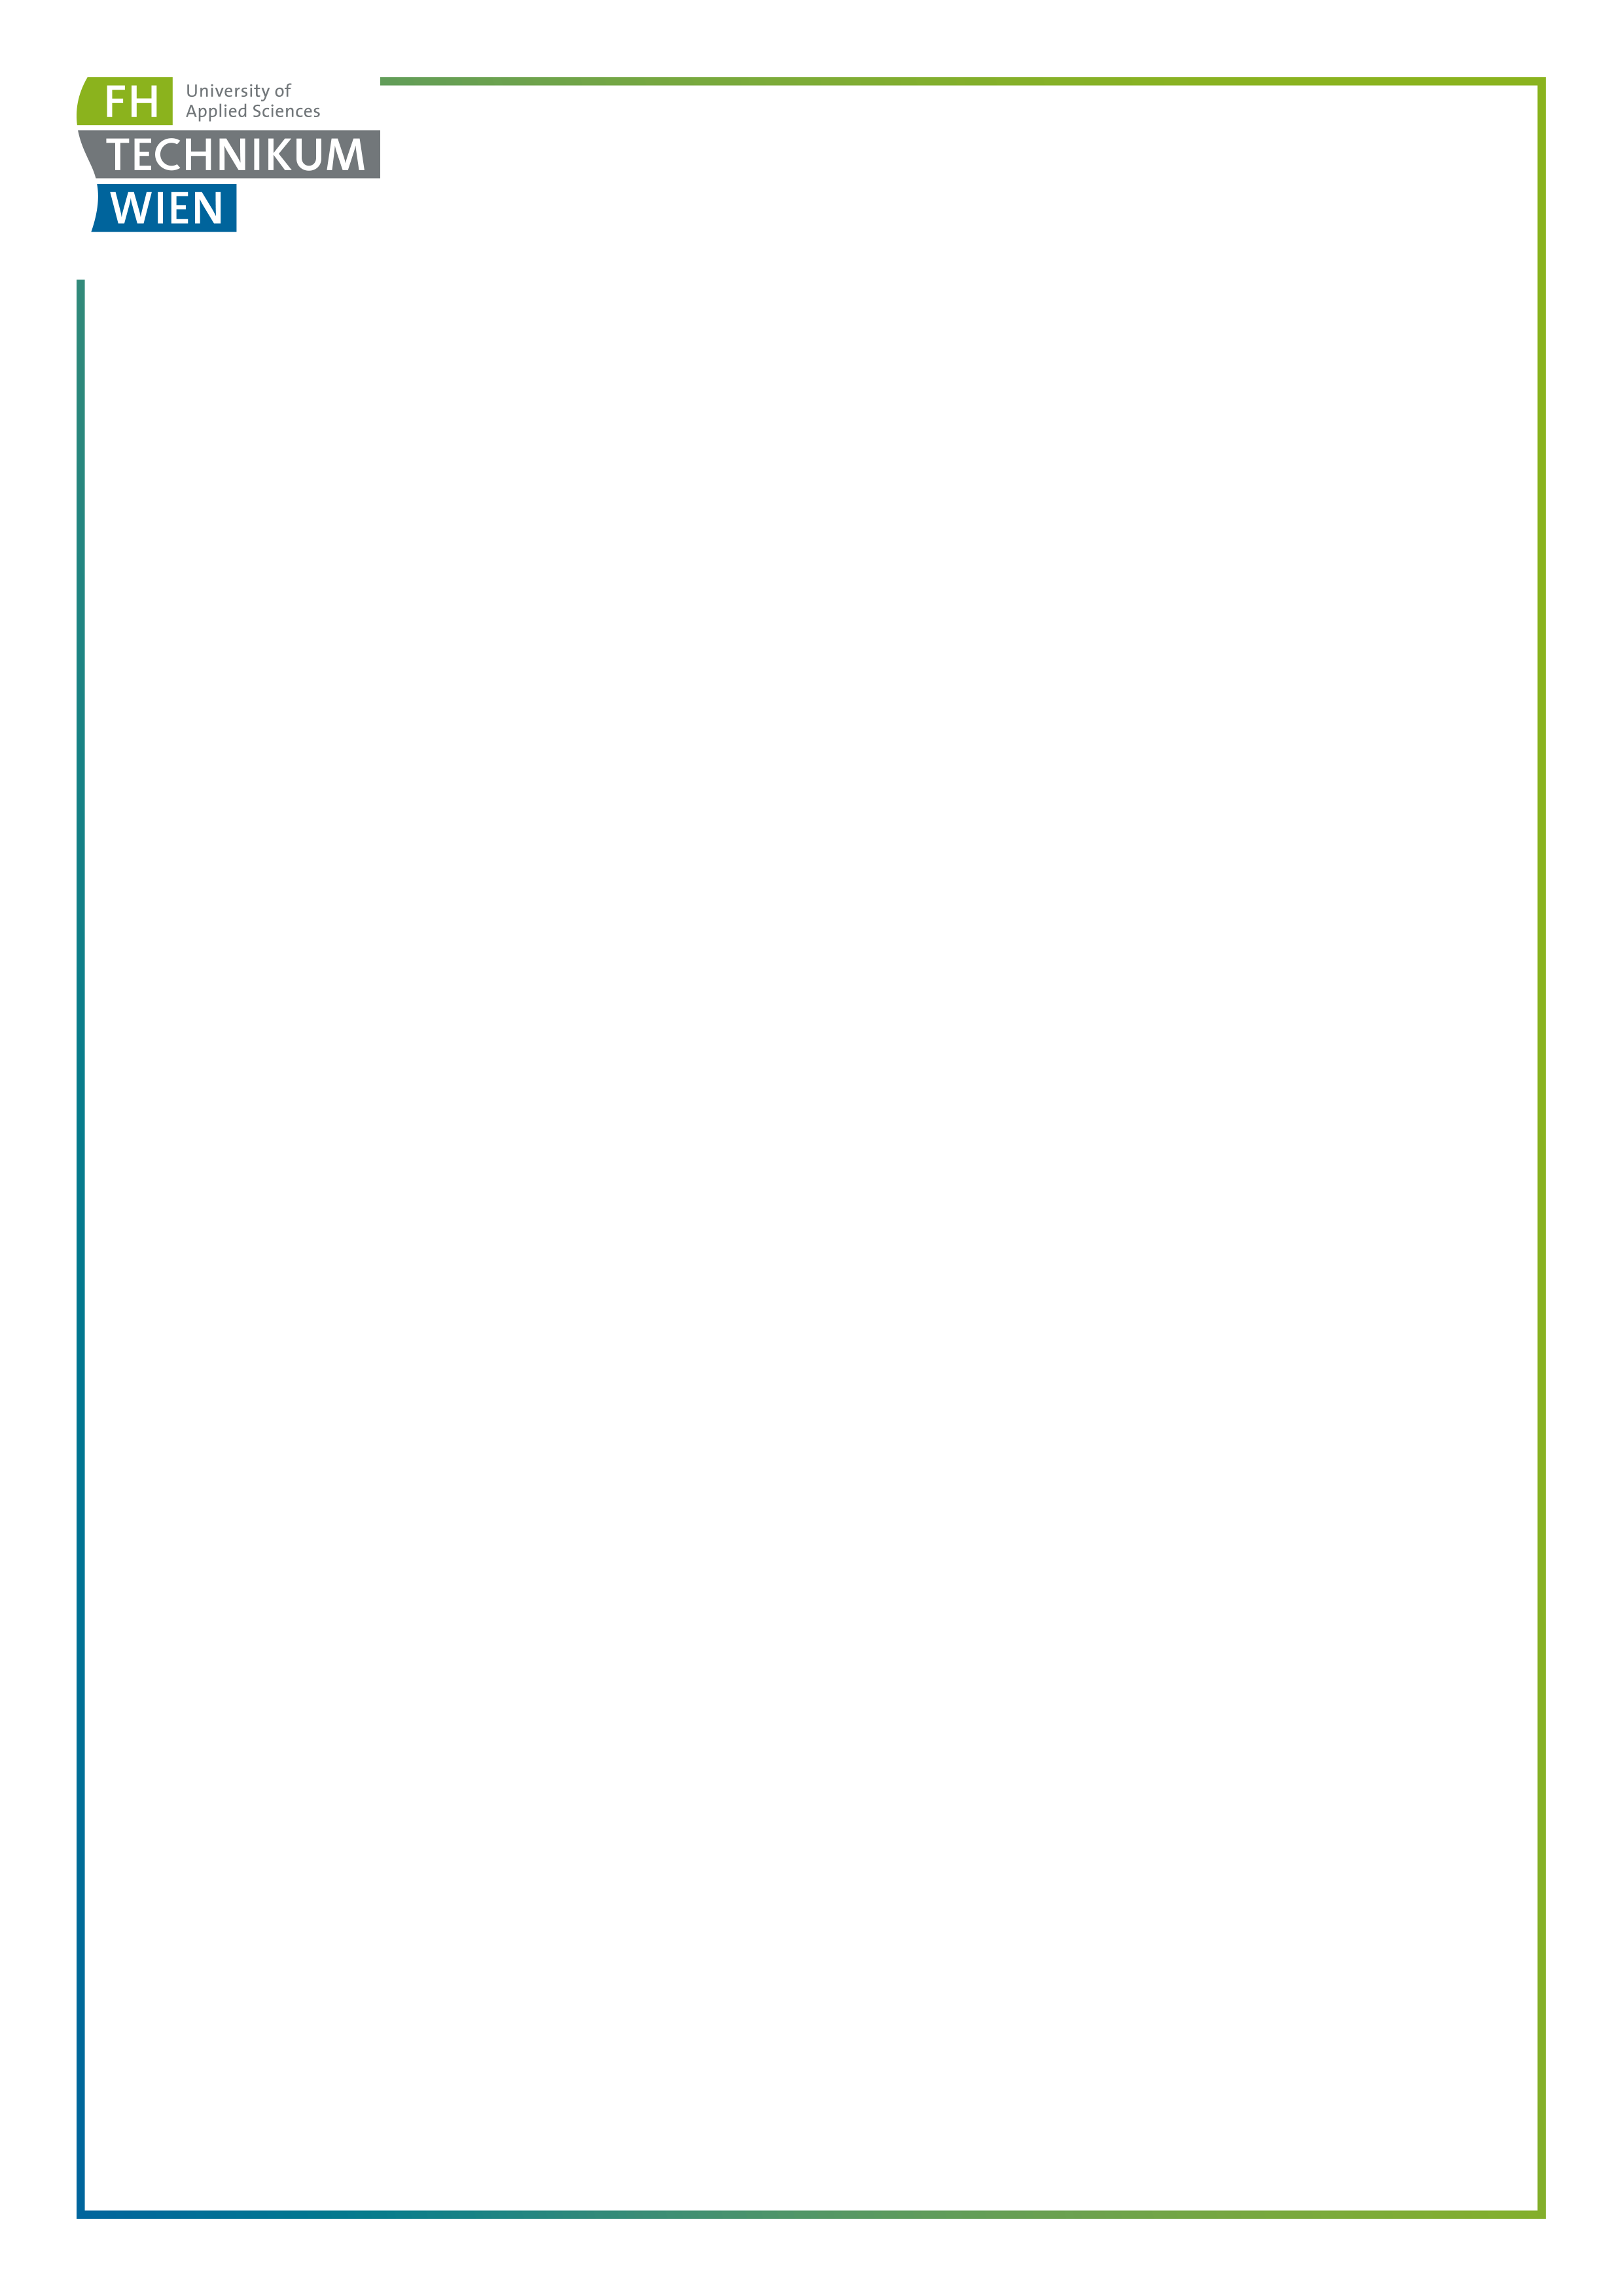
\includegraphics[width=0\linewidth]{PICs/fhtw_cover}
\clearpage


\end{document}
